\documentclass[a4paper, 12pt]{report}
\usepackage[a4paper,hmargin={1.25in, 1in},vmargin={1in, 1in}]{geometry}
\usepackage{amsfonts} % if you want blackboard bold symbols e.g. for real numbers
\usepackage{graphicx} % if you want to include jpeg or pdf pictures
\usepackage{cite}
\usepackage{booktabs}
\usepackage[english]{babel}
\addto {\captionsenglish}{
\renewcommand*{\bibname}{References}
\renewcommand*{\tocname}{References}
}
\usepackage[autostyle, english = american]{csquotes}
\usepackage{multicol}
\usepackage{lipsum}
\usepackage{subfig}
\usepackage{setspace}
\usepackage{float}
\usepackage{blindtext}
\usepackage{fancyhdr}
\usepackage{tikz}
\usepackage{titlesec}
\usetikzlibrary{calc}
\usepackage{setspace}
\usepackage{eso-pic}
\usepackage{lipsum}
\usepackage{times}
\usepackage[nottoc]{tocbibind}
\usepackage{}
\newcommand{\bsp}{\begin{spacing}{1.5}}
\newcommand{\esp}{\end{spacing}}
\pagestyle{fancy}
\fancyhf{}
\lhead{}
\renewcommand{\footrulewidth}{0.4pt}
\rhead{\textit{{Brain Tumor Detection using Machine Learning Approach}}}
\rfoot{\thepage}
\fancypagestyle{custom}{
\fancyhf{}
\fancyhead[R]{\textit{Brain Tumor Detection using Machine Learning Approach}}
\fancyhead[R]{\thepage}
}
%\titleformat{\chapter}[display]
%  {\fontsize{16}{14}\bfseries\huge}
%{}
%  {0pt}
%  {\filcenter}
%\titleformat{\section}[block]
%  {\fontsize{14}{14}\bfseries}
%  {\thesection}
%  {1em}
%  {\MakeUppercase}
%\titleformat{\subsection}[block]
%  {\fontsize{12}{14}\bfseries}
%  {\thesubsection}
%  {1ex}
 % {}%
 
{\titleformat{\chapter}[hang]
{\filleft\huge\bfseries}{\chaptertitlename\ \thechapter:}{20pt}{\Huge}
\titlespacing*{\chapter}{0pt}{-25pt}{20pt}
\begin{document}
%========================================================= %
%================begin of title page====================== %
% The frontmatter environment for everything that comes with roman numbering\
%============================================= %
\newenvironment{frontmatter}{}{}
\begin{frontmatter}
%%%%%%%%%%%%%%%%%%%%%%%%%%%%%%%%%%%%%%%%%%%%%%%%%%%%%%%%%%%%%%%%%%%
\begin{titlepage}
%\AddToShipoutPictureBG
\begin{center}
\textup{\large  \textbf{Savitribai Phule Pune University}\\\textbf{Modern Education Society\rq s College of Engineering, Pune}}\\19, Bund Garden, V.K. Joag Path, Pune – 411001. \\[0.2cm]\textbf{ACCREDITED BY NAAC WITH {\lq\lq A\rq\rq} GRADE}\\[0.2cm]\textbf{\large DEPARTMENT OF COMPUTER ENGINEERING}
%---------------------------------Figure------------------------------
\begin{center}
\begin{figure}[h]  %h means here other options t , b, p, etc.
\centering

\includegraphics[width=0.3\linewidth]{./logo1}
\end{figure}
\end{center}
%----------------------------
\textup{\large  A \\ [0.4cm] SEMINAR REPORT\\[0.4cm]ON}\\[0.4cm]
\begin{LARGE}
{\textbf {\lq\lq BRAIN TUMOR DETECTION USING\vspace*{0.1in} MACHINE LEARNING APPROACH\rq\rq}}\end{LARGE}\\[1.2cm]
\begin{large}\textbf {T.E. (COMPUTER ENGINEERING)}
\end{large}\\[1cm]
\textit{SUBMITTED BY}\\[0.5cm]

\textbf{SUDESH PAWAR}\\
{\small\textbf{SEAT NO:71818502B}}\\[0.7cm]

\textit{GUIDED BY}\\[0.5cm]
\begin{large}\textbf{Prof. Jayshree R. Pansare}\\[0.3cm]\end{large}
\textbf{(Academic Year: 2019-2020)}
\vfill
\end{center}
\end{titlepage}
%================begin of certificate page======================
\begin{titlepage}
\begin{tikzpicture}[overlay,remember picture]
\draw[line width=4pt]
    ($ (current page.north west) + (1cm,-1cm) $)
    rectangle
    ($ (current page.south east) + (-1cm,1cm) $);
\draw[line width=1.5pt]
    ($ (current page.north west) + (1.2cm,-1.2cm) $)
    rectangle
    ($ (current page.south east) + (-1.2cm,1.2cm) $);
\end{tikzpicture}
\begin{center}
\textup{\large \textbf{Modern Education Society\rq s College of Engineering, Pune}}\\19, Bund Garden, V.K. Joag Path, Pune – 411001.\\[0.8cm]\textbf{ACCREDITED BY NAAC WITH {\lq\lq A\rq\rq} GRADE}\\[0.8cm]\textbf{\large DEPARTMENT OF COMPUTER ENGINEERING}
%---------------------------------Figure-----------------
\begin{figure}[h]
\centering

\includegraphics[width=0.3\linewidth]{./logo1}
\end{figure}
%-------------------------------------------------------
\\
\begin{LARGE}
\textbf{\textit {CERTIFICATE}}\end{LARGE}\\[1.2cm]
\textit{This is to certify that seminar entitled}\\[0.5cm]\large\textbf{\lq\lq Brain Tumor Detection using Machine Learning Approach\rq\rq}
\end{center}  
has been completed by Mr. Sudesh Pawar, Seat No:71818502B of TE COMP-I in the Semester-II of academic year 2019-2020 in partial fulfillment of the Third Year of Bachelor degree in \lq\lq Computer Engineering\rq\rq as prescribed by the Savitribai Phule Pune University.
\vspace{3cm}
\begin{multicols}{2}
\begin{flushleft}
\textbf{Dr. Jayshree R. Pansare}\hspace{5cm}\\
\textbf{Seminar Guide}\\
\end{flushleft}
\begin{flushright}
\textbf{Dr. (Mrs.) N. F. Shaikh\\ { HOD}}\\
\end{flushright}
\end{multicols}\vspace{0.6cm}
\flushleft
\textit{Place:}MESCOE,Pune.\\
\textit{Date:}\hspace{0.4cm}   /\hspace{0.4cm}  /2020
\vfill
\end{titlepage}
%================end of title page======================
%----------------------ACKNOWLEDGEMENT---------------------------
\pagebreak
\renewcommand{\baselinestretch}{1.5}
\newpage
\begin{center}
{\Large{\bf{\textit{ACKNOWLEDGEMENT}}\\[2cm]}}
\end{center}
\par \textit{\quad \quad It gives me great pleasure and satisfaction in presenting this seminar on \lq\lq Brain Tumor Detection using Machine Learning Approach\rq\rq.}
\par \textit{\quad \quad I would like to express my deep sense of gratitude towards {\bf Dr. Jayshree R. Pansare} for her untiring guidance, constant supervision, enthusiastic encouragement, sagacious advice and an effective surveillance throughout the entire period of my seminar.}
\par \textit{\quad \quad I have furthermore to thank Computer Department HOD }{\bf Dr. (Mrs.) N. F. Shaikh}\textit{, \quad \quad Principal }{\bf Dr.A.A. Keste}  \textit{to encourage me to go ahead and for continuous guidance}.

\par \textit{\quad \quad I would like to thank all those, who have directly or indirectly helped me for the completion of the work during this seminar.}
\vspace{0.8in}
\begin{flushright}
{SUDESH PAWAR}\\
\hspace*{0.1in}{T.E. Computer Engineering}\\
\hspace*{0.1in}{Seat no. : 71818502B}\\
\end{flushright}



\newpage
\tableofcontents
\listoffigures
\listoftables
\lfoot{Department of Computer Engineering, MESCOE, Pune}
%\vspace{cm}
%%%%%%%%%%%%%%% Abstract %%%%%%%%%%
\newpage
\begin{center}
{\Large{\bf Abstract}}
\end{center}

Nowadays, Brain Tumor Detection has turned up as a important parameter in the realm of health care. Brain tumor can be denoted as a ill-shaped tissue wherein the cells multiply abruptly and there is no control over the growth of the cells. The process of Image Segmentation is adopted for extracting abnormal tumor region within the brain. In the Magnetic Resonance Image, segmentation of brain tissue holds very significant in order to identify the presence of outlines concerning the brain tumor. There is abundance of uncovered information in stored in the Health care sector. With appropriate use of accurate data mining classification techniques, early prediction of any disease can be effectively performed. In the medical field, the techniques of ML and Data mining holds a significant stand. Majority of which is adopted effectively. Also the method proposed assures to be efficient and precise for brain tumor detection, classification and segmentation. To achieve this precise automatic or semiautomatic methods are needed. The research proposes an automated segmentation method that relies upon CNN, determining small 3 x 3 kernels. By incorporating this single technique, segmentation and classification is accomplished. CNN wherein it has layer based for results classification. Various levels involved in the proposed mechanisms are: Data collection, Pre-processing,Aver age filtering, Segmentation, Feature Extraction, CNN via Classification and Identification. By utilizing the Data mining techniques, significant relations and patterns from the data can be extracted. The techniques of ML and Data mining are being effectively employed for brain tumor detection and prevention at an early stage.\\
[1cm]
{\textbf{Keywords}}:\textit{ Abnormalities; Magnetic Resonance Imaging; Brain Tumor; Pre-processing; Segmentation; Feature Extraction; ML techniques; Data Mining; CNN}
\vspace{0.3cm}
%================================================ %
% The frontmatter environment for everything that comes with roman numbering %
\end{frontmatter}
%%%%%%%%%%%%%%%%%%%%%%%%%%%%%%%%%%%%%%%

\newpage
%%%%%%%%% MAIN TEXT STARTS HERE %%%%%%%%%%
\begin{spacing}{1.5}
\chapter{INTRODUCTION} 

\section{BRAIN TUMORS - A Brief History}

\par Tumor basically symbolizes abnormal, uncontrollable growth of cells within the body. Brain tumor signifies an abnormal tissue wherein the cells multiply abruptly within the brain tissues \cite{alic}.Brain tumor segmentation involves separating distinct tumor cells (effective tumor, solid, edema, and necrosis) from the grey matter, white matter, and cerebrospinal fluid. Concerning Brain Tumor Research, the unnatural cells tend to be explored any time \cite{nellyg}. The procedure of MRI doesn’t involve any pain or radiation and is a non-invasive imaging process \cite{ayun}. Early diagnosis and treatment of brain tumor definitely increases the survival chances of an individual. Using DM, abundant data can be analyzed from various angles thus extracting valuable information. The system focuses on to build a diagnosis and prediction system related to brain tumor by incorporating predictive mining. Brain tumor can be related to numerous medical comorbidities. These abnormal medical symptoms has a direct impact on the brain. Presently, it is considered as a foremost health issue.\\

\section{Brief Introduction to the System}
\par The survey examines all risk factors that are being traced out in brain tumor surveillance systems. Also the method proposed assures to be efficient and precise
for brain tumor detection, classification and segmentation. For these reasons, accurate methods are required. The system proposes an automated segmentation method that relies upon CNN, determining 3 x 3 kernels. By incorporating this, segmentation and classification is accomplished. The system proposes a novel tumor detection technique on the basis of high-level extracted features from CNNs making use of Hough transform technique. The tumors that are being detected, undergoes segmentation using a set of fully connected layers, thereafter, the segmented mask is classified. The proposed approach yields outcome as per the standard medical imaging benchmarks. CNN is a deep learning algorithm adopted to examine the Image. It utilizes various multilayer perceptions framed to gain comparatively reduced pre -processing time. The processes involved in the proposed approach being: Data collection, Pre-processing, then comes the Average filtering which presents and identifies the clarity image and thereafter the segmentation process for pixel based detection, segmentation concerning the brain image and other areas being affected, next is the process of feature extraction extracts various feature such as PSNR, MEAN, Entropy, standard deviations etc... By utilizing data mining, significant relations and patterns can be found. The techniques of ML and Data mining are being effectively employed for brain tumor detection and prevention at an early stage. Literature Survey, proposed approach for detection of Brain tumor and aspects of various levels, outcome, discussion and the conclusion are discussed in further sections.\\

\subsection{Requirements for Machine Learning}
\subsubsection{Hardware Requirements}

You won’t need a high-end gaming set or Supercomputer to do Machine Learning.What you require is:-

\begin{enumerate}
 \item Intel Core i5-7200U processor or better
 \item 8GB of DDR3 RAM or better
 \item 10GB of free disk space
 \item DX12-capable GPU to train ML Model
 \item HDMI 1.4 or DisplayPort 1.2
\end{enumerate}

\subsubsection{Software Requirements}
You will have to fulfill the following software requirements:-
\begin{enumerate}
\item Python 3
\item Windows 10(Any Version)
\end{enumerate}

\newpage
\chapter{LITERATURE SURVEY}

\par C.Hemasundara Rao et.al, suggests an automated method for detection and segmenting affected areas. Proposed method suggests: initial segmentation, Modelling and Optimizing the energy function. The information present in T1, FLAIR MRI images are being utilized for effective segmentation. Conditional random field-based framework is employed to merge information existing in T1 and FLAIR in probabilistic region.\cite{chema} Atiq Islam et.al suggests using the multi-fractal feature extraction and enhanced AdaBoost classification schemes for detection and segmentation. By making use of feature extraction strategy, the tumor texture is extracted. This is a higly complex scheme.\cite{atiq}\\

\par Meiyan Huang et.al suggests using the local independent projection-based classification for classifying voxel and extracting path feature. Explicit regularization not required. Less accurate method\cite{meiy}. Bjoern H. Menze et.al, presents multimodal brain tumor segmentation scheme. Various segmentation algorithm are being combined to gain better performance. Though, it is still complex \cite{bjoe}.\\

\par  Shamsul Huda et.al presents hybrid feature selection using ensemble classification for performing tumor diagnosis. For acquiring of decision rules, Decision Tree, GANNIGMAC, Bagging C based wrapper approach are adopted and the decision rules are simplified by making use of hybrid feature selection.\cite{smsl}. Sergio Pereira et.al presents automated methods for identification and type cataloging by utilizing MRI of Brain right from when one could attempt a scan in the computer system. On the contrary, Neural Networks and SVM are used as they offer better performance \cite{sergio}.\\

\par J. Seetha et.al, suggests use of MRI images for the diagnosis. The scan usually produces huge data which makes the manual classification process slow. Therefore, automated and trustworthy classification to reduce the human death ratio needed. Automated classification is very complex in some areas. Herein, proposed an automated detection approach by adopting CNN classification \cite{jsit}. N.V. Shree et.al, targets on noise removal, extraction of gray-level co-occurrence matrix features, tumor region growing segmentation for minimizing complexity and enhanced performance. Later, morphological filtering is used to remove noise built up. Classifier is being utilized for training and testing. \cite{nvs}.\\

\par Z. Tang et.al, presents Multi-atlas segmentation for MRI of Brain. MAS basically works by registering and fusing label information from numerous normal brain atlases into a new brain image for the process of segmentation. Mostly it is framed for normal images, though the tumor brain images remains a challenge. For resolving this, at the initial level, a new low-rank method is being adopted for retrieving the recovered image of normal brain from the MR tumor brain image relying upon normal brain information. In the next step, normal brain atlases are being registered for recovering the image.\cite{zhen}.

\par B. Singh et.al, suggests process of pre-processing wherein there is noise elimination by employing fuzzy filter and mean shift based fuzzy c-means algorithm which requires low computation and offers better segmentation output. The above techniques has a mean field phrase in the traditional fuzzy c-means objective function. Since it’s possible for the mean shift to locate cluster centers quiet
easily and promptly, all the techniques can carry out effective diagnosis\cite{balj}.

\par GarimaSingh et.al, presents a technique to classify and analyze with de-noising filters like the Adaptive filter, Median filter, Un-sharp masking filter, Averaging filter and Gaussian filter that are employed to eliminate additive noises in the MRI images which includes: speckle noise, Gaussian, Salt and pepper noise. For successful tumor identification, using normalized histogram and segmentation via K-means clustering suggested. Naïve Bayes Classifier and SVM are adopted for classifying the MRIs, thereby offering precise prediction and classification \cite{gari}.

\par G. Rajesh Chandra et.al, suggests soft thresholding DWT for improvisation and genetic
algorithms for the purpose of segmentation. The proposed approach utilizes the potential of GA for resolving
optimization issues with a large search space. Also, the proposed method integrates any prior available knowledge. The established method obtained SNR value ranging from (20 to 44) and segmentation accuracy from (82 to 97 pc) related to detected tumor pixels on the basis of ground truth \cite{grc}.

\chapter{METHODOLOGY}

\section{System Architecture}

\par Brain tumor basically symbolizes abnormal and uncontrollable growth of cells within the brain. Basically it’s of two types: first being the malignant tumor that contains cancerous cells and second one is the benign tumor which doesn’t have any cancerous cells. Convolution Neural Networks consists of multiple layers of responsive fields. The technique of Brain tumor segmentation is based on CNN by determining small 3 x 3 kernels. Utilization of small kernels allows for an indepth architecture, apart from posing a positive impact in contrast to over-fitting, with minimum type of masses existing in the network. At the same time inspecting the employment of intensity normalization as a preprocessing process. It’s imbibed in combination with information segmentation, being intolerable against neoplasm segmentation concerning the MR imaging picture.\\

\begin{figure}[h!]
\centering
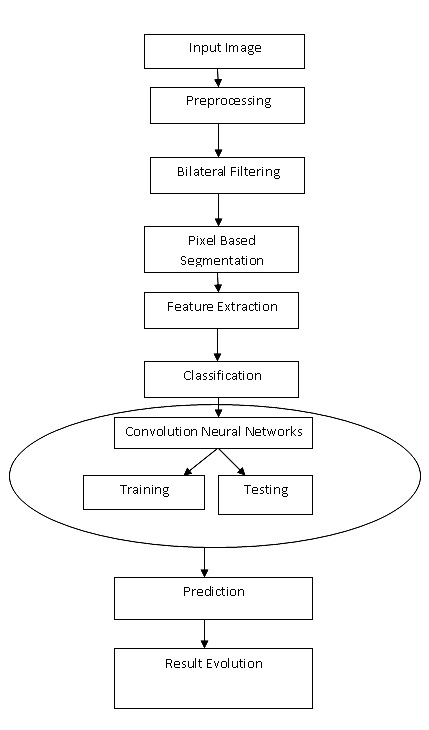
\includegraphics[width=0.8\linewidth]{sysarch.jpg}
\caption{Proposed Architecture}
\end{figure}


\newpage
\section{Brain Image Processing}

\par Due to existing noise in the Magnetic Resonance, images get affected. For noise reduction, the system proposes local smoothing methods and nonlocal means. In the image there maybe significant structures and details that can act as noise; they are eliminated too. Pre-processing involves steps like data cleaning, data transformation, data integration, data resizing, data reduction etc. 
\par The image pre-processing eliminates unnecessary data and smooth up noise, detect and eliminate the outlier and rectify the inconsistencies. Lastly, normalization and aggregation is performed. The technique of Image-processing proves to be highly significant in determining particular image, removing noise and for improvising the quality.

\section{Average Filtering}
\par The normal channel being the convolution work that is utilized to set the clamor in the images. The Preprocessing step abandons the disturbances but still after applying it the image doesn’t hold suitable for future process. Therefore, the Average channel resolves this issue by providing acceptable and smooth picture. The Average channel resembles a non-linear channel unlike straight channels. It replace the pixel esteems with an Average esteem that being nearly accessible. Moreover, Average channel tends to be edge safeguarding. It helps in abandoning salt and pepper disorder in the images.\\

\textbf{Algorithm for Filtering}:
\begin{enumerate}
	\item The picture is provided as input.
	\item Choose a 3X3 window near the current pixel within the picture.
	\item Perform pixel sorting in expanding request and save it to a vector.
	\item Determine the normal of the vector.
	\item The current pixel is replaced with the normal esteem.
	\item Repetition of Steps 2 to 5 till every single pixels within the picture gets prepared.
	\item Output.
\end{enumerate}

\section{Pixel based Segmentation}
\par Image Segmentation is a common technique of digital image processing. Lately, Brain tumor image sectioning in MRI has spurred up as a popular research in the domain of medical imaging system. The process of Segmentation helps a lot to simplify the detection of malignant and benign tumors.

\section{Convolutional Neural Networks}
\par Convolutional Neural Network is employed for segmenting the images. It directly extracts features from pixel images with least pre-processing involved. The network utilized is LinkNet which being a light deep neural network architecture that’s developed to carry out semantic segmentation. It contains encoder and decoder blocks which basically manage to split the image and re-build again before it’s forwarded via few final convolutional layers. CNN is a significant approach of deep learning which is being employed in image recognition. It involves 2 basic methods: convolution and pooling. Convolution and pooling layers are arranged till high level of classification accuracy is achieved. Moreover, few feature maps are identified in every convolutional layer and weights linked to it are being shared. This offer comprehension of various network characteristics at the same time retaining the no. of traceable parameters. CNN possess less specific tasks in contrast to the conventional methods and helps in thoroughly extracting features.\\

\begin{figure}[h!]
	\centering
	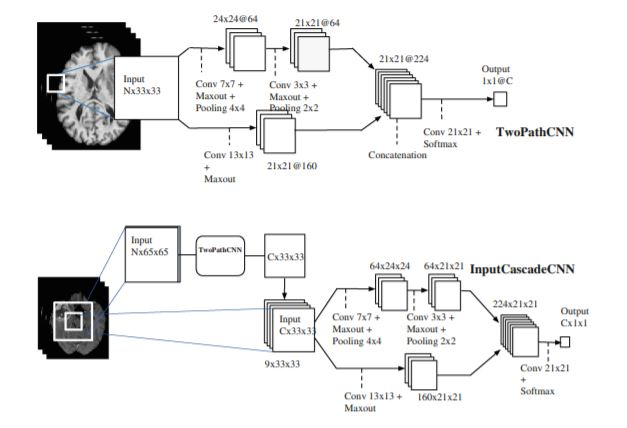
\includegraphics[width=0.8\linewidth]{CNN.jpg}
	\caption{CNN Architecture}
\end{figure}

\textbf{Algorithm for CNN based Classification:}
\begin{enumerate}
	\item Convolution filter is applied in the first layer..
	\item The filter sensitivity is minimized by smoothing the conv filter (by sub-sampling).
	\item The Activation layer controls the signal transfer from one layer to other layer.
	\item Training period is being fastened by employing RELU (rectified linear unit).
	\item The neurons in proceeding layer is associated with each neuron in the next layer.
	\item At the time of training, Loss layer is appended in the end to provide a feedback to NN (neural network).
\end{enumerate}

\section{Evolution Metrics}

\par For performance evaluation and measuring system stability, few parameters are computed and examined. These are mentioned as:
\par The proposed CNNs performance is assessed with Root Mean Square Error, recall, sensitivity, precision, F-score specificity, probability of the misclassification error and accuracy of the training and testing set and throughout performance was examined by
making use of the Equations correspondingly, where Yi denotes actual and Ri denotes result of the ith diagnosis of brain tumor feature acquired, TN (True Negative) denotes
prediction for the patients with no brain tumor and were detected with no brain tumor, FN (False Negative) denotes the prediction for the patients with no brain tumor but
were detected with a brain tumor, TP(True Positive) denotes the prediction for the patients with brain tumor and were detected with a brain tumor, and FP(False Positive) represents the prediction for the patients having brain tumor but were detected with no brain tumor.

\section{Result and Discussion}
\par The proposed method employs a mean field term within standard CNN objective function. The technique is developed and applied in MATLAB environment by utilizing the image processing tool. Datasets are assembled from the UCI datasets. A comparison is found among all the features and the entire result being depicted in the figures. The accuracy is computed which is then compared with rest of the methods. Efficiency and training accuracy of the proposed brain tumor classification approach is computed.\\

\par Table 1 illustrates the comparison of various classification techniques. It represents overall performance and comparison output in contrast to various prevailing techniques such as CRF, SVM and GA. The proposed CNN (Convolutional Neural Network)yields in improvised output in contrast to the
existing algorithms.

\begin{table}[h!]
	\centering
	\begin{tabular}{||c|c|c|c||}
		\hline
		S.No & Techniques & Accuracy(\%) & Efficiency(\%)\\
		[0.5ex]
		\hline \hline
		1 & Conditional Random Field(CRF) & 89 & 87.5 \\
		2 & Support Vector Machine (SVM) & 84.5 & 90.3 \\
		3 & Genetic Algorithm (GA) & 83.64 & 84.78 \\
		4 & Convolutinal Neural Network(CNN) & 91 & 92.7\\ [1ex]
		\hline
	\end{tabular}
	\caption{Comparison of Classification Techniques}
	\label{table:1}
\end{table}
\subsection{Simulation Results}

\par The datasets are accumulated from online datasets and the MATLAB environment is used for the development process. Figures presented below depicts the overall images of brain tumor detection. Input image undergoes pre-processing. Thereafter the pre-processed image is enhanced and the image is extracted. Eventually, the brain tumor classified image is retrieved and implemented successfully.
\newpage
\begin{figure}[h]
\centering
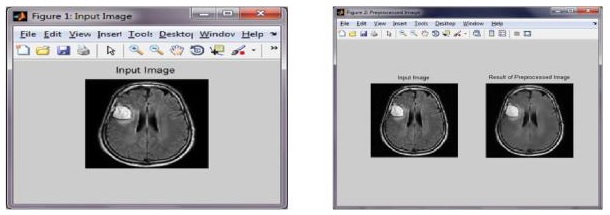
\includegraphics[width=0.7\linewidth]{./ippre}
\caption{Input and Preprocessed Image}
\end{figure}

\begin{figure}[h]
	\centering
	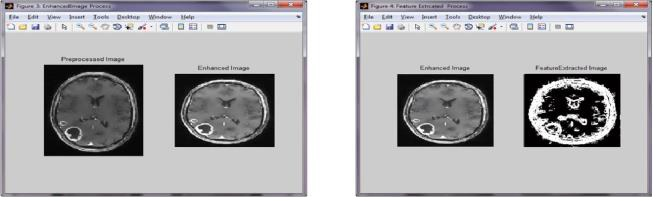
\includegraphics[width=0.7\linewidth]{./efe}
	\caption{Enhanced and Feature-Extracted Image}
\end{figure}

\begin{figure}[h]
	\centering
	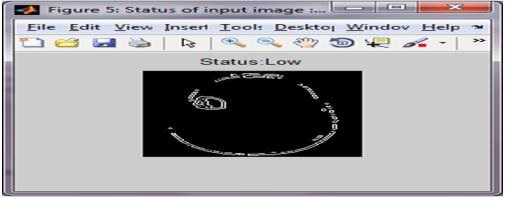
\includegraphics[width=0.7\linewidth]{./classified}
	\caption{Classified Image}
\end{figure}
\newpage

\chapter{CONCLUSION}
\par Referring the earlier section, it is revealed that output generated is quiet accurate. Accuracy achieved at the end relies upon each step and processing done in it. There are lot
of existing methods for every step, hence the methods that give optimum results are selected. At the last, Brain Tumor Classification takes place. To detect Brain Tumor Detection there exist different standard approaches but the present work utilizes the traditional Neural Network approach for detecting the brain tumor, since the brain tumor detection images relies upon the neighborhood pixels.\\
\par The CNN approach discussed provides powerful brain tumor detection. The proposed algorithm is implemented on multiple images present in the dataset and the output retrieved is best and effective.\\
\label{References}
\bibliography{repcite}
\bibliographystyle{ieeetr}
\end{spacing}

\end{document} 
%
